% !TEX encoding = UTF-8
% !TEX TS-program = pdflatex
% !TEX root = ../tesi.tex
% !TEX spellcheck = it-IT

%**************************************************************
\chapter{Progettazione e codifica}
\label{cap:progettazione-codifica}
%**************************************************************

\intro{In questo capitolo verrà descritta la progettazione dell'ultimo prototipo}\\


\section{Metodo e formalismo di specifica}
Nell'esposizione dell'architettura del prodotto si procederà con un approccio di tipo top-down.  Si descriverà quindi l'architettura iniziando dal generale ed andando al particolare; descrivendo prima i componenti, per poi descrivere nel dettaglio le singole classi.\\

Per ogni componente saranno descritti brevemente il tipo, l'obiettivo e la funzione e saranno specificati
eventuali figli, classi ed interazioni con altri componenti. Ogni classe sarà dotata di una breve descrizione e
ne saranno specificate le responsabilità, le classi ereditate, le sottoclassi e le relazioni con altre classi.\\
Infine si illustreranno degli esempi di utilizzo dei \emph{design pattern} nell'architettura del sistema.

\section{Legenda}
Tutti i diagrammi usano la convenzione di colori descritta nella legenda in figura~\ref{fig:legenda} al fine di migliorare la leggibilità. I livelli di annidamento sono da intendere per la totale struttura dei package e non solo per il singolo schema.\\
Si noti in particolare che le classi e componenti di colore arancio rappresentano classi di librerie esterne al sistema, ma vengono talora rappresentate comunque per maggiore chiarezza.
\begin{figure}[H] 
    \centering 
    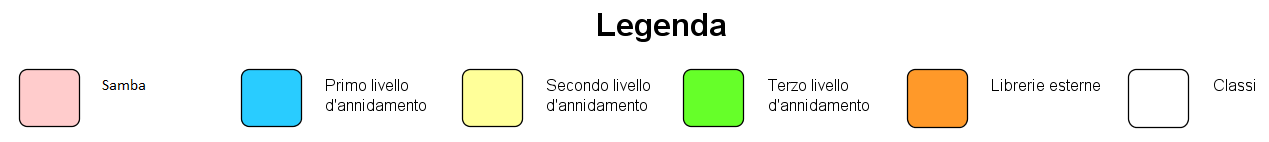
\includegraphics[width=0.9\columnwidth]{varie/Legenda.png} 
    \caption{Legenda}\label{fig:legenda}
\end{figure}


\section{Architettura generale}




%**************************************************************
\section{Componenti e classi}

\subsection{Samba}
\begin{figure}[!h] 
    \centering 
    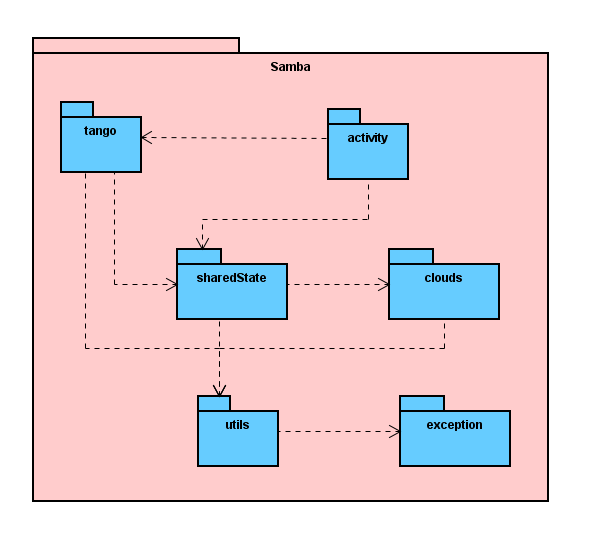
\includegraphics[width=0.9\columnwidth]{st/Samba.png} 
    \caption{Componente Samba}\label{fig:comp-Samba}
\end{figure}
\subsubsection{Descrizione}
È il livello principale del sistema lato \emph{tablet}.
\subsubsection{Package figli}
\begin{itemize}
	\item Samba.activity
	\item Samba.tango
	\item Samba.sharedState
	\item Samba.clouds
	\item Samba.utils
	\item Samba.exception
\end{itemize}

\subsection{Samba.activity}
\begin{figure}[!h] 
    \centering 
    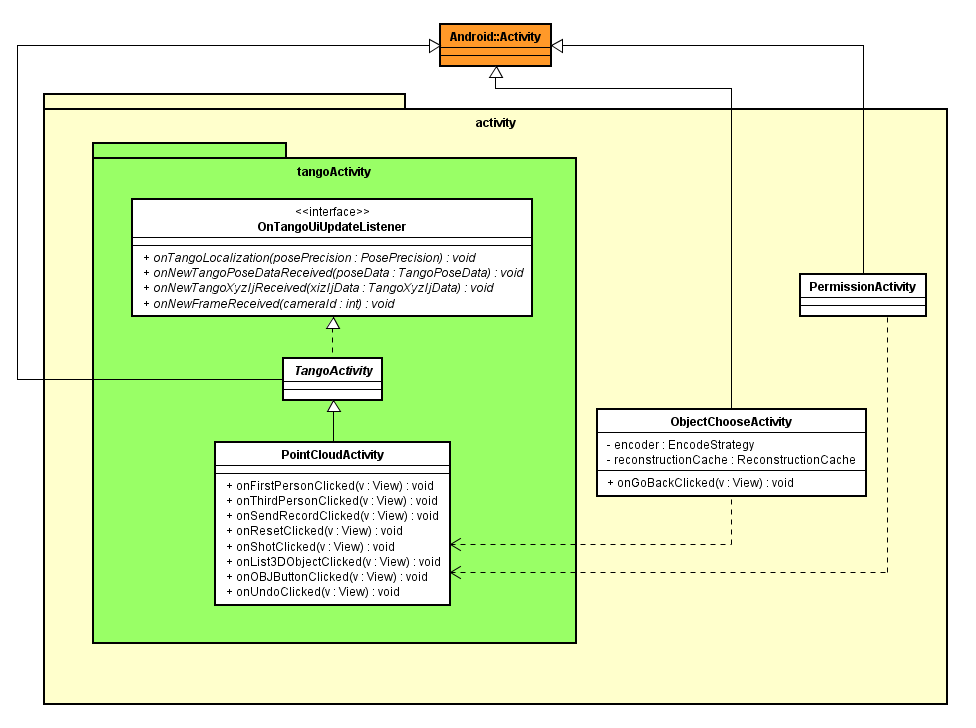
\includegraphics[width=1.0\columnwidth]{st/Samba_activity.png} 
    \caption{Componente Samba.activity}
\end{figure}
\subsubsection{Descrizione}
Questo \emph{package} contiene tutte le \emph{activity} necessarie per l'applicazione. Contiene inoltre la definizione di una interfaccia per le attività che vogliono fare uso dei vari \emph{manager} messi a disposizione (si veda sezione \ref{subs:samba-tango}).
\subsubsection{Package figli}
\begin{itemize}
	\item Samba.activity.tangoActivity
\end{itemize}
\subsubsection{Classi}
\begin{itemize}
	\item Samba.activity.PermissionActivity
	\item Samba.activity.ObjectChooseActivity
\end{itemize}

\subsection{Samba.activity.tangoActivity}
\subsubsection{Descrizione}
Questo \emph{package} serve a contenere tutte le \emph{activity} che vogliono essere attività Tango, ovvero che vogliono poter usare i \emph{manager} messi a disposizione (si veda sezione \ref{subs:samba-tango}).
\subsubsection{Interfacce}
\begin{itemize}
	\item Samba.activity.tangoActivity.OnTangoUiUpdateListener
\end{itemize}
\subsubsection{Classi}
\begin{itemize}
	\item Samba.activity.tangoActivity.TangoActivity
	\item Samba.activity.tangoActivity.PointCloudActivity
\end{itemize}

\subsection{Samba.activity.tangoActivity.OnTangoUiUpdateListener}
\subsubsection{Descrizione}
Interfaccia che deve essere implementata da tutte le \emph{activity} che vogliono fare uso dei \emph{manager Tango} messi a disposizione (si veda sezione \ref{subs:samba-tango}). Espone metodi pubblici che possono essere chiamati da altre componenti quando avranno la necessità di notificare qualche cambiamento di stato.
\subsubsection{Utilizzo}
Viene implementate dalle \emph{activity} che vogliono interagire con il ciclo di vita dei sensori \emph{Tango}. Verrà usata per permettere indirettamente alle componenti che gestiscono i sensori \emph{Tango} di aggiornare la \emph{UI}.
\subsubsection{Implementata da}
\begin{itemize}
	\item Samba.activity.tangoActivity.TangoActivity
\end{itemize}

\subsection{Samba.activity.tangoActivity.TangoActivity}
\subsubsection{Descrizione}
Classe astratta che estende \emph{Activity} e implementa l'interfaccia che fornisce i \emph{callback} necessari per permettere ai componenti che interagiscono con il ciclo di vita dei sensori \emph{Tango} di modificare indirettamente la \emph{UI}.
\subsubsection{Utilizzo}
È utilizzata come superclasse astratta di tutte le attività che vogliono interagire con i sensori \emph{Tango}.
\subsubsection{Relazioni con altre classi}
\begin{itemize}
	\item \texttt{Samba.sharedState.ReconstructionManager}: relazione entrante, dipendenza, utilizzo come parametro di uno o più metodi.
	\item \texttt{Samba.tango.CloudRecorder}: relazione entrante, dipendenza, utilizzo come parametro di uno o più metodi.
	\item \texttt{Samba.tango.RajawaliRendererManager}: relazione entrante, dipendenza, utilizzo come parametro di uno o più metodi.
	\item \texttt{Samba.tango.RGBBoxManager}: relazione entrante, dipendenza, utilizzo come parametro di uno o più metodi.
	\item \texttt{Samba.tango.TangoManager}: relazione entrante, dipendenza, utilizzo come parametro di uno o più metodi.
\end{itemize}
\subsubsection{Estesa da}
\begin{itemize}
	\item Samba.activity.tangoActivity.PointCloudActivity
\end{itemize}
\subsubsection{Interfacce implementate}
\begin{itemize}
	\item Samba.activity.tangoActivity.OnTangoUiUpdateListener
\end{itemize}
\subsubsection{Classi estese}
\begin{itemize}
	\item android.app.Activity
\end{itemize}

\subsection{Samba.activity.tangoActivity.PointCloudActivity}
\subsubsection{Descrizione}
Attività principale dell'applicazione prodotta: fornisce un \emph{render} dei punti, una \emph{preview} della fotocamera e pulsanti per accedere a tutte le altre funzionalità dell'applicazione.\\
\subsubsection{Utilizzo}
È usata per gestire il ciclo di vita dell'\emph{activity} principale dell'applicazione.
\subsubsection{Relazioni con altre classi}
\begin{itemize}
	\item \texttt{Samba.activity.ObjectChooseActivity}: relazione entrante, dipendenza, utilizzo della classe per costruire un \emph{Intent}.
	\item \texttt{Samba.activity.PermissionActivity}: relazione entrante, dipendenza, utilizzo della classe per costruire un \emph{Intent}.
	\item \texttt{Samba.sharedState.ReconstructionCache}: relazione uscente, composizione.
	\item \texttt{Samba.sharedState.ReconstructionManager}: relazione uscente, composizione.	
	\item \texttt{Samba.tango.TangoManager}: relazione uscente, composizione.
	\item \texttt{Samba.tango.RajawaliRendererManager}: relazione uscente, composizione.
	\item \texttt{Samba.tango.RGBBoxManager}: relazione uscente, composizione.
\end{itemize}
\subsubsection{Classi estese}
\begin{itemize}
	\item Samba.activity.tangoActivity.TangoActivity
\end{itemize}

\subsection{Samba.activity.ObjectChooseActivity}
\subsubsection{Descrizione}
Attività che può leggere e scrivere su disco, compila la lista dei \emph{File pcd} salvati e permette all'utente di compiere diverse azioni su questi ultimi.
\subsubsection{Utilizzo}
Viene usata quando l'utente richiede di visualizzare la lista dei \emph{file pcd} salvati su disco, oppure quando vuole caricarli/eliminarli/spedirli al \emph{Server}.
\subsubsection{Relazioni con altre classi}
\begin{itemize}
	\item \texttt{Samba.activity.tangoActivity.PointCloudActivity}: relazione uscente, dipendenza, utilizzo della classe per costruire un \emph{Intent}.
\end{itemize}
\subsubsection{Classi estese}
\begin{itemize}
	\item android.app.Activity
\end{itemize}

\subsection{Samba.activity.PermissionActivity}
\subsubsection{Descrizione}
Attività che ha il solo compito di richiedere all'utente i permessi di utilizzare l'\emph{Area Learning}. \emph{Google} fornire un \emph{Intent} apposito per ottenere tali permessi ed essi devono essere assolutamente garantiti dall'utente prima dell'inizio del processo di localizzazione. Per questo sono richiesti in una attività a parte e che viene lanciata precedentemente rispetto all'attività principale.
\subsubsection{Utilizzo}
Viene lanciata ad ogni avvio dell'applicazione allo scopo di richiedere i permessi, in caso l'utente non li abbia ancora garantiti, controllarne la presenza altrimenti.
\subsubsection{Relazioni con altre classi}
\begin{itemize}
	\item \texttt{Samba.activity.tangoActivity.PointCloudActivity}: relazione uscente, dipendenza, utilizzo della classe per costruire un \emph{Intent}.
\end{itemize}
\subsubsection{Classi estese}
\begin{itemize}
	\item android.app.Activity
\end{itemize}

\subsection{Samba.tango}\label{subs:samba-tango}
\begin{figure}[!h] 
    \centering 
    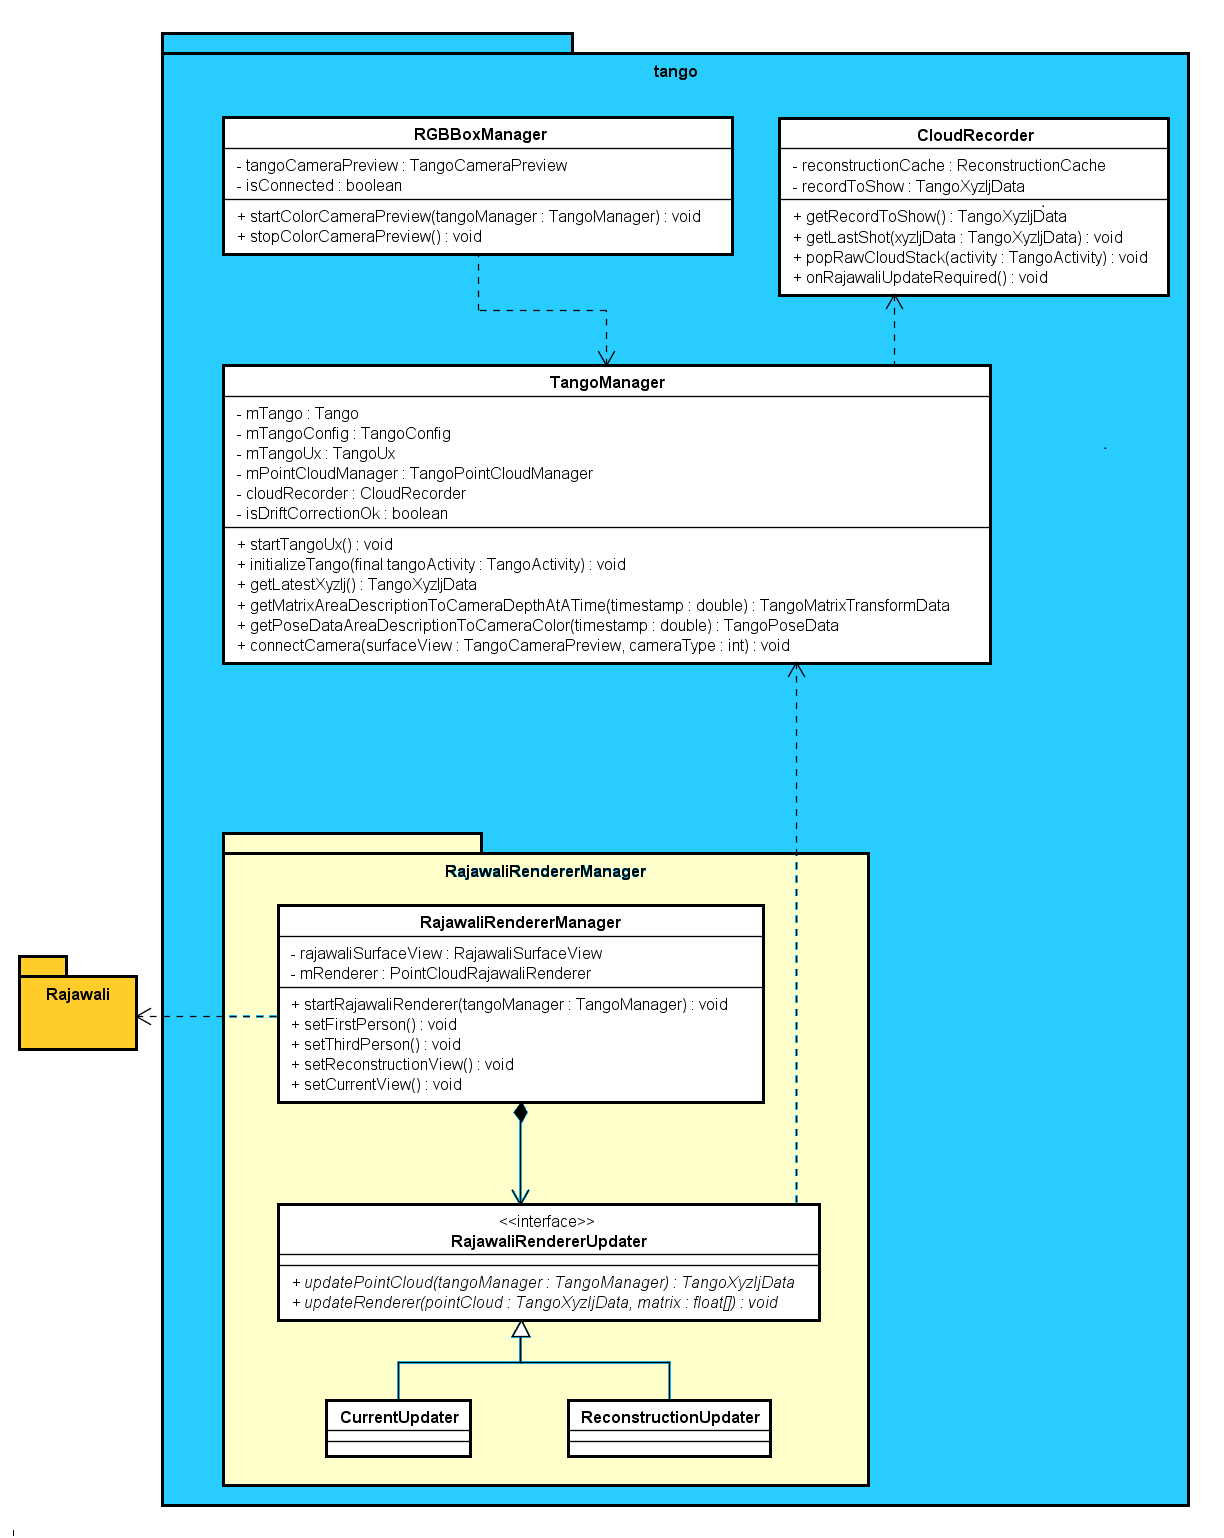
\includegraphics[width=1.0\columnwidth]{st/Samba_tango.png} 
    \caption{Componente Samba.tango}
\end{figure}
\subsubsection{Descrizione}
Questo \emph{package} contiene un insieme di classi che possono essere usate per interagire con il ciclo di vita dei sensori \emph{Tango} e del \emph{renderer} dei punti. Questi \emph{manager} possono essere usati per gestire la \emph{business logic} di una applicazione \emph{Tango} separandola dalla sua rappresentazione grafica.
\subsubsection{Package figli}
\begin{itemize}
	\item Samba.tango.RajawaliRendererManager
\end{itemize}
\subsubsection{Classi}
\begin{itemize}
	\item Samba.tango.RGBBoxManager
	\item Samba.tango.CloudRecorder
	\item Samba.tango.TangoManager
\end{itemize}

\subsection{Samba.tango.RajawaliRendererManager}
\subsubsection{Descrizione}
\emph{Package} che contiene il \emph{manager} per gestire il \emph{rendering} dei punti tramite la libreria \emph{Rajawali}.
\subsubsection{Interfacce}
\begin{itemize}
	\item Samba.tango.RajawaliRendererManager.RajawaliRendererUpdater
\end{itemize}
\subsubsection{Classi}
\begin{itemize}
	\item Samba.tango.RajawaliRendererManager.RajawaliRendererManager
	\item Samba.tango.RajawaliRendererManager.CurrentUpdater
	\item Samba.tango.RajawaliRendererManager.ReconstructionUpdater
\end{itemize}


\subsection{Samba.tango.RajawaliRendererManager.RajawaliRendererManager}
\subsubsection{Descrizione}
Questa classe permette di integrare un servizio di \emph{rendering} di \emph{Point Cloud} all'interno del ciclo di vita di una applicazione \emph{Andorid}. Oltre alla visualizzazione espone metodi per cambiare la modalità del \emph{render}, e di effettuare qualche azione sullo stesso.
\subsubsection{Utilizzo}
È utilizzata per fornire un \emph{render} nell'attività principale dell'applicazione prodotta. (Come quello in figura \ref{fig:render-rajawali} in tutta la parte destra dello schermo)
\subsubsection{Relazioni con altre classi}
\begin{itemize}
	\item \texttt{Samba.activity.tangoActivity.PointCloudActivity}: relazione entrante, composizione.
	\item \texttt{Samba.activity.tangoActivity.TangoActivity}: relazione uscente, dipendenza, utilizzo come parametro di uno o più metodi.
	\item \texttt{Samba.tango.RajawaliRendererManager.RajawaliRendererUpdater}: relazione uscente, composizione.
\end{itemize}

\subsection{Samba.tango.RajawaliRendererManager.RajawaliRendererUpdater}
\subsubsection{Descrizione}
Interfaccia che rappresenta il componente \emph{Strategy} del \emph{Desing Pattern} \emph{Strategy}.
\subsubsection{Utilizzo}
È usata per alternare la modalità del \emph{render} tra la rappresentazione in tempo reale dei dati del sensore e quella della ricostruzione corrente.
\subsubsection{Relazioni con altre classi}
\begin{itemize}
	\item \texttt{Samba.tango.RajawaliRendererManager.RajawaliRendererManager}: relazione entrante, composizione.
	\item \texttt{Samba.tango.TangoManager}: relazione uscente, dipendenza.
\end{itemize}
\subsubsection{Implementata da}
\begin{itemize}
	\item Samba.tango.RajawaliRendererManager.CurrentUpdater
	\item Samba.tango.RajawaliRendererManager.ReconstructionUpdater
\end{itemize}


\subsection{Samba.tango.RajawaliRendererManager.CurrentUpdater}
\subsubsection{Descrizione}
Implementazione di \emph{RajawaliRendererUpdater} che rappresenta la visione in tempo reale dei dati del sensore.
\subsubsection{Utilizzo}
È usata per impostare il \emph{render} alla modalità in tempo reale.
\subsubsection{Interfacce implementate}
\begin{itemize}
	\item Samba.tango.RajawaliRendererManager.RajawaliRendererUpdater
\end{itemize}

\subsection{Samba.tango.RajawaliRendererManager.ReconstructionUpdater}
\subsubsection{Descrizione}
Implementazione di \emph{RajawaliRendererUpdater} che rappresenta la visione del \emph{Point Cloud} correntemente ricostruito.
\subsubsection{Utilizzo}
È usata per impostare il \emph{render} alla modalità ricostruzione.
\subsubsection{Interfacce implementate}
\begin{itemize}
	\item Samba.tango.RajawaliRendererManager.RajawaliRendererUpdater
\end{itemize}

\subsection{Samba.tango.RGBBoxManager}
\subsubsection{Descrizione}
Questa classe permette di integrare un servizio di \emph{preview} della fotocamera all'interno del ciclo di vita di una applicazione \emph{Andorid}.
\subsubsection{Utilizzo}
È utilizzata per fornire una \emph{preview} della fotocamera nell'attività principale dell'applicazione prodotta. (Come quella in figura \ref{fig:render-rajawali} in basso a sinistra)
\subsubsection{Relazioni con altre classi}
\begin{itemize}
	\item \texttt{Samba.activity.tangoActivity.PointCloudActivity}: relazione entrante, composizione.
	\item \texttt{Samba.activity.tangoActivity.TangoActivity}: relazione uscente, dipendenza, utilizzo come parametro di uno o più metodi.
	\item \texttt{Samba.tango.TangoManager}: relazione uscente, dipendenza.
\end{itemize}

\subsection{Samba.tango.TangoManager}
\subsubsection{Descrizione}
Questa classe permette di integrare i servizi \emph{Tango} all'interno del ciclo di vita di una applicazione \emph{Andorid}. Inoltre imposta correttamente il \emph{framework} \emph{TangoUx} e fornisce metodi per ricavare statistiche e dati algebrici.
\subsubsection{Utilizzo}
È utilizzata per fornire all'attività principale dell'applicazione prodotta la possibilità di sfruttare i servizi \emph{Tango}.
\subsubsection{Relazioni con altre classi}
\begin{itemize}
	\item \texttt{Samba.activity.tangoActivity.PointCloudActivity}: relazione entrante, composizione.
	\item \texttt{Samba.activity.tangoActivity.TangoActivity}: relazione uscente, dipendenza, utilizzo come parametro di uno o più metodi.
	\item \texttt{Samba.tango.RGBBoxManager}: relazione entrante, dipendenza.
	\item \texttt{Samba.tango.RajawaliRendererManager.RajawaliRendererUpdater}: relazione entrante, dipendenza.
	\item \texttt{Samba.tango.CloudRecorder}: relazione uscente, dipendenza.
	\item \texttt{Samba.clouds.utils.poseSanity.PoseSanityChecker}: relazione uscente, composizione.
\end{itemize}

\subsection{Samba.tango.CloudRecorder}
\subsubsection{Descrizione}
Mantiene la ricostruzione corrente in un formato comprensibile dal \emph{renderer}.
\subsubsection{Utilizzo}
Viene usata per effettuare il \emph{rendering} del \emph{Point Cloud} della ricostruzione corrente.
\subsubsection{Relazioni con altre classi}
\begin{itemize}
	\item \texttt{Samba.activity.tangoActivity.PointCloudActivity}: relazione entrante, composizione.
	\item \texttt{Samba.activity.tangoActivity.TangoActivity}: relazione uscente, dipendenza, utilizzo come parametro di uno o più metodi.
	\item \texttt{Samba.tango.TangoManager}: relazione entrante, dipendenza.
	\item \textbf{Samba.sharedState.ReconstructionCache}: relazione uscente, composizione.
\end{itemize}


\subsection{Samba.sharedState}
\begin{figure}[!h] 
    \centering 
    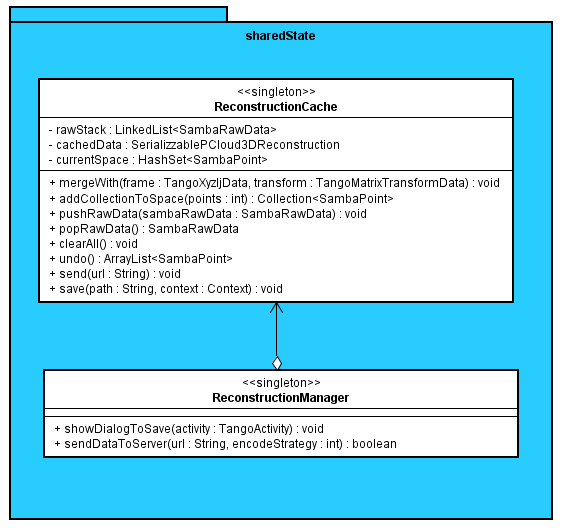
\includegraphics[width=0.9\columnwidth]{st/Samba_sharedState.png} 
    \caption{Componente Samba.sharedState}
\end{figure}
\subsubsection{Descrizione}
Questo \emph{package} contiene un \emph{singleton} che mantiene tutti gli stati condivisi tra i vari servizi e una classe di utilità.
\subsubsection{Classi}
\begin{itemize}
	\item Samba.sharedState.ReconstructionCache
	\item Samba.sharedState.ReconstructionManager
\end{itemize}

\subsection{Samba.sharedState.ReconstructionCache}
\subsubsection{Descrizione}
Questo \emph{singleton} mantiene tutte le informazioni condivise tra i vari servizi asincroni presenti nell'applicazione. Fornisce tutti i metodi necessari per accedervi controllatamente, e si occupa anche di sincronizzare gli accessi stessi dove necessario.
\subsubsection{Utilizzo}
È usata dai servizi presenti nell'applicazione per salvare e modificare i loro stati condivisi.
\subsubsection{Relazioni con altre classi}
\begin{itemize}
	\item \texttt{Samba.sharedState.ReconstructionManager}: relazione entrante, aggregazione.
	\item \texttt{Samba.activity.ObjectChooseActivity}: relazione entrante, composizione.
	\item \texttt{Samba.activity.tangoActivity.PointCloudActivity}: relazione entrante, composizione.
	\item \texttt{Samba.tango.CloudRecorder}: relazione entrante, composizione.
	\item \texttt{Samba.utils.services.MergingService}: relazione entrante, composizione.
	\item \texttt{Samba.utils.services.VoxelService}: relazione entrante, composizione.	
\end{itemize}

\subsection{Samba.sharedState.ReconstructionManager}
\subsubsection{Descrizione}
\emph{Singleton} di utilità che fornisce delle \emph{macro} per sequenze di operazioni effettuate ricorrentemente su \emph{ReconstructionCache}.
\subsubsection{Utilizzo}
Viene usato da alcuni componenti per effettuare complesse operazioni sullo stato condiviso.
\subsubsection{Relazioni con altre classi}
\begin{itemize}
	\item \texttt{Samba.sharedState.ReconstructionCache}: relazione uscente, aggregazione.
	\item \texttt{Samba.activity.tangoActivity.PointCloudActivity}: relazione entrante, composizione.	
\end{itemize}


\subsection{Samba.clouds}
\begin{figure}[!h] 
    \centering 
    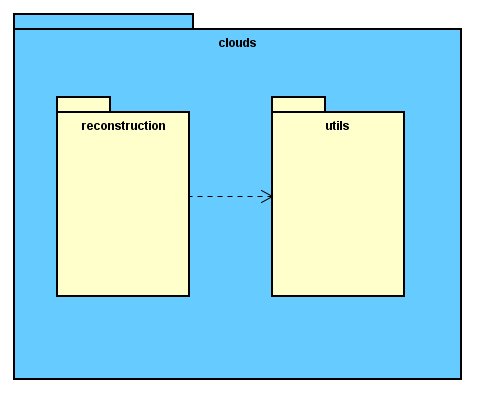
\includegraphics[width=0.8\columnwidth]{st/Samba_clouds.png} 
    \caption{Componente Samba.clouds}
\end{figure}
\subsubsection{Descrizione}
Questo \emph{package} contiene tutte le strutture dati usate per rappresentare internamente i \emph{Point Cloud}.
\subsubsection{Package figli}
\begin{itemize}
	\item Samba.clouds.reconstruction
	\item Samba.clouds.utils
\end{itemize}


\subsection{Samba.clouds.reconstruction}
\begin{figure}[!h] 
    \centering 
    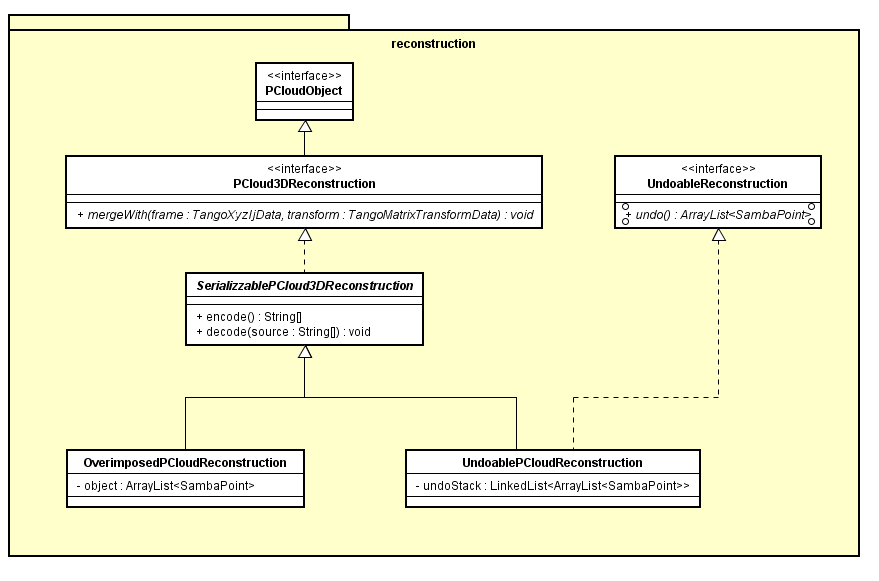
\includegraphics[width=1.0\columnwidth]{st/Samba_clouds_reconstruction.png} 
    \caption{Componente Samba.}
\end{figure}
\subsubsection{Descrizione}
Per motivi di ottimizzazione si è cercato di lasciare il più possibile aperte le possibilità di modifica della rappresentazione interna dei \emph{Point Cloud} ricostruiti. Questo \emph{package} contiene tutte le classi che rappresenta un \emph{Point Cloud} ricostruito.
\subsubsection{Interfacce}
\begin{itemize}
	\item Samba.clouds.PCloudObject
	\item Samba.clouds.PCloud3DReconstruction
	\item Samba.clouds.UndoableReconstruction
\end{itemize}
\subsubsection{Classi}
\begin{itemize}
	\item Samba.clouds.OverimposedPCloudReconstruction
	\item Samba.clouds.UndoablePCloudReconstruction
\end{itemize}



\ \\ \ \\ \ \\ \ \\ \ \\ \ \\ \ \\ \ \\




%\subsection{Samba.sharedState.}
%\subsubsection{Descrizione}
%\subsubsection{Utilizzo}
%\subsubsection{Relazioni con altre classi}
%\begin{itemize}
%	\item \texttt{Samba.}:
%\end{itemize}
%\subsubsection{Classi estese}
%\begin{itemize}
%	\item Samba.
%\end{itemize}
%
%
%\subsection{}
%\begin{figure}[!h] 
%    \centering 
%    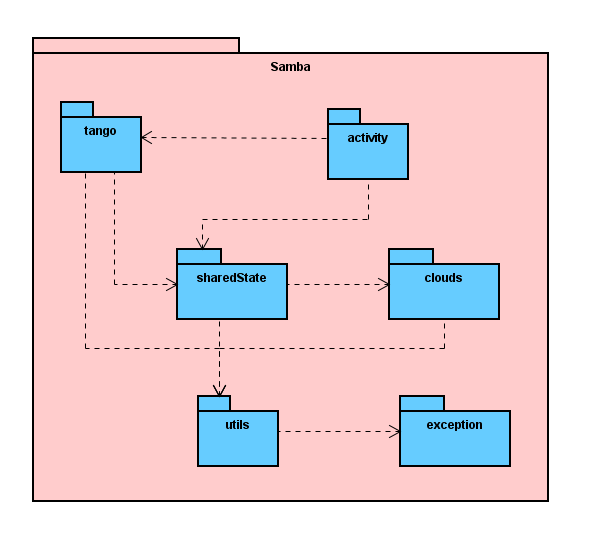
\includegraphics[width=1.0\columnwidth]{st/Samba.png} 
%    \caption{Componente Samba.}
%\end{figure}
%\subsubsection{Descrizione}
%\subsubsection{Package figli}
%\begin{itemize}
%	\item Samba.
%\end{itemize}
%\subsubsection{Classi}
%\begin{itemize}
%	\item Samba.
%\end{itemize}



%**************************************************************
\section{Design Pattern utilizzati}

%**************************************************************
\section{Codifica}
